\documentclass[10pt,twocolumn, nofootinbib]{revtex4-1}
%\documentclass[aps,pra,10pt,twocolumn,floatfix,nofootinbib]{revtex4-1}
%\documentclass[10pt,twocolumn,letterpaper]{article}

\usepackage{amsmath}
\usepackage{amssymb}
\usepackage{graphicx}
\usepackage{amsfonts}
\usepackage{enumitem}
\usepackage{graphicx}
\usepackage{hyperref}
\usepackage{tikz}

\hypersetup{
	colorlinks=true,
	citecolor=blue,
	urlcolor=blue,
	linkcolor=blue
}
\urlstyle{same}
\frenchspacing

\newcommand\partitle[1]{\textsc{#1}.}


\begin{document}

\title{On the reality of the quantum state once again: A no-go theorem for $\psi$-ontic models}
\author{Gabriele Carcassi}
\affiliation{Physics Department, University of Michigan, Ann Arbor, MI 48109}
\author{Andrea Oldofredi}
\affiliation{Centre of Philosophy, University of Lisbon, Portugal}
\author{Christine A. Aidala}
\affiliation{Physics Department, University of Michigan, Ann Arbor, MI 48109}
\vspace{2mm}

\date{\today}


\begin{abstract}
In 2010 Harrigan and Spekkens (HS) proposed a rigorous classification in order to categorize the nature of the quantum state, i.e.\ to establish whether in a certain model $\psi$ corresponds to a real property of a quantum object, in which case the model is called $\psi$-ontic, or to some observer information, making it $\psi$-epistemic. Building on the HS framework Pusey, Barrett and Rudolph (PBR) proved a theorem claiming that $\psi$-epistemic models contradict quantum mechanics, and thus quantum states cannot be taken to represent mere information about quantum systems. In this essay we propose a simple no-go theorem that explains why also $\psi$-ontic models cannot be expected to reproduce quantum mechanics. We will see that, using information theoretic considerations, the lack of overlap of epistemic states requires all states to be orthogonal, which openly contradicts quantum theory. Combining our result with the PBR argument, our conclusion is that both $\psi$-epistemic and $\psi$-ontic models contradict quantum mechanics. 
\end{abstract}

\maketitle

\section{Introduction}
 
In 2010 Harrigan and Spekkens (HS) proposed a rigorous classification in order to categorize the nature of the quantum state, i.e.\ to establish whether in a certain model $\psi$ corresponds to a real property of a quantum object, in which case the model is called $\psi$-ontic, or to some observer information, making it $\psi$-epistemic \cite{Harrigan:2010}. While their original aim was to clarify Einstein's view of Quantum Mechanics (QM), the HS framework has been widely employed in the literature not only to categorize different formulations of QM, but also to argue what types of interpretations are admissible (\cite{Leifer:2013, Leifer:2017, Branciard:2014, Hermens:2021, Wood:2015, Ringbauer:2015, Mazurek:2016, Bartlett:2012}; cf.\ \cite{Oldofredi:2020b, Ladyman:2021} for critical discussions). 

Referring to this, one of the most influential works based on HS classification is due to Pusey, Barrett and Rudolph who published a formal result in \emph{Nature Physics}---widely known as the PBR theorem---showing that ``if the quantum state merely represents information about the real physical state of a system, then experimental predictions are obtained that contradict those of quantum theory'' (\cite{PBR:2012}, p.\ 475). Alternatively stated, PBR argued that in every model reproducing the statistics and predictions of QM the quantum state $\psi$ must represent real physical properties of the system under consideration and not agents' knowledge---i.e.\ models must be $\psi$-ontic. Consequently, quantum theories cannot be $\psi$-epistemic. 

Such a theorem had a remarkable resonance (\cite{Leifer:2014, Leifer:2014b, Lewis:2012, Renner:2012, Colbeck:2017, Hardy:2013, Maroney:2014, Patra:2013, Mansfield:2016, Schlosshauer:2012, Schlosshauer:2013, Schlosshauer:2014, Aaronson:2013}), and questions about its actual meaning are still discussed today: on the one hand, it rules out interpretations of QM where $\psi$ merely represents information. On the other, scholars recently showed that non-trivial epistemic as well as statistical approaches to QM are not refuted by the PBR argument (\cite{Ben:2017, Rizzi:2018, Oldofredi:2021, DeBrota:2019}).

In this paper we are not going to rebut the theorem itself. We instead aim to carefully re-examine one of its premises, i.e.\ HS classification between $\psi$-ontic and $\psi$-epistemic ontological models on top of which the PBR result is derived. We believe that a careful analysis of this assumption forces us to re-evaluate the significance of this classification as well as the meaning of the PBR conclusion. In other words, we re-examine the definitions and features of such models in order to understand whether they constitute a sound basis from which to draw conclusions on the nature of $\psi$, given the influence that the HS framework has in quantum foundations. As the reader will see, our analysis suggests that they are not.

While the PBR theorem is a no-go result for $\psi$-epistemic models, in this essay we provide a no-go theorem for $\psi$-ontic models: using information theoretic considerations we show that $\psi$-ontic models cannot reproduce all the predictions, results and implications of QM since the lack of overlap of epistemic states---a necessary condition for a model to be $\psi$-ontic---requires that all states must be orthogonal, which openly contradicts quantum theory. Therefore, we conclude, $\psi$-ontic models should not be employed in order to classify quantum theories. 

Combining our result with the PBR argument, we conclude that the HS classification itself is fundamentally empty, i.e.\ both $\psi$-epistemic and $\psi$-ontic models do contradict quantum mechanics. Consequently, HS framework should be employed neither to classify interpretations of the quantum formalism, nor to draw conclusion about the nature of $\psi$. 

\section{Summary of the Harrigan \& Spekkens Model}

We briefly review the main features of the classification provided by HS starting with the usual operational setting for QM. We have a preparation protocol $P$, associated with a density operator $\rho$ on the relevant Hilbert space, and a measurement protocol $M$, represented by a POVM $\{ E_k\}$ where each $k$ represents a possible measurement outcome. The probability of obtaining a particular $k$ given a particular preparation $P$ and measurement $M$ is given by the generalized Born rule
\begin{equation}
	p(k|M, P)=\textrm{tr}(\rho E_k).
\end{equation}

An ontological model, as defined by HS, additionally assumes that there exists a set of states $\Lambda$, called \textbf{ontic states}, that provide the complete specification of the properties of a given physical object. A preparation $P$ will prepare a particular ontic state $\lambda$ according to the probability distribution $p(\lambda | P)$, which is referred to as \textbf{epistemic state}. The measurement outcome will depend only on the ontic state with probability $p(k|\lambda, M)$ (\cite{Harrigan:2010}, p.\ 128). This leads to the following expression:
\begin{equation}
	\int_\Lambda d\lambda p(k|\lambda, M) p(\lambda| P)= \textrm{tr}(\rho E_k).
\end{equation}
It is also assumed that a mixture of pure states $\{ \psi_i \}$ with probabilities $\{ w_i \}$ will be represented by
\begin{equation}\label{epistemic_mixing}
	\sum_i  w_i p(\lambda| P_{\psi_i}).
\end{equation}
As the epistemic states for mixed preparations are simply linear combinations of epistemic states for pure preparations, the HS model concentrates on the latter.

To classify an ontological model, we look at the relationship between quantum and ontic states. There are two broad categories. In a \textbf{$\psi$-ontic} model the wave function is a physical property of the ontic state, in the sense that given an ontic state $\lambda$ there is only one pure state preparation $P_\psi$ that could have prepared $\lambda$. As we can see in figure \ref{overlap} (a), this happens if the probability distributions do not overlap, i.e.\ if we have
\begin{equation}\label{ontic_condition}
	p(\lambda | P_{\psi})p(\lambda|P_{\phi})=0
\end{equation}
for all pairs of states $\psi$ and $\phi$. If a model is not $\psi$-ontic, then it is \textbf{$\psi$-epistemic}. In this case, $\lambda$ can be described by more than one quantum state and the wave function is taken to represent knowledge about the state preparation---in such models quantum states generate overlapping probability distributions over $\Lambda$ as shown in figure \ref{overlap} (b). A $\psi$-ontic model is said \textbf{$\psi$-complete} if the quantum states and the ontic states coincide. More precisely if 
\begin{equation}\label{complete_condition}
	p(\lambda|P_\psi)=\delta(\lambda-\lambda_{\psi}).
\end{equation}
All other models are \textbf{$\psi$-incomplete}.

To make this classification more concrete, let us give an example from classical mechanics. Consider the case where we prepare a particle according to a specific value of energy. The energy partitions phase space into mutually exclusive regions, and therefore we can understand the energy of the preparation as a property of the particle itself. According to HS, this would be an \emph{ontic property}. Consider now the case where we prepare a particle according to a specific temperature. When we take the particle from the oven, we are sampling from a Boltzmann distribution over different energies. However, unlike energy, temperature does not partition phase space because the same particle state could have been prepared by ovens at different temperature. Temperature is a property of the preparation and therefore an \emph{epistemic property}. 

\begin{figure}
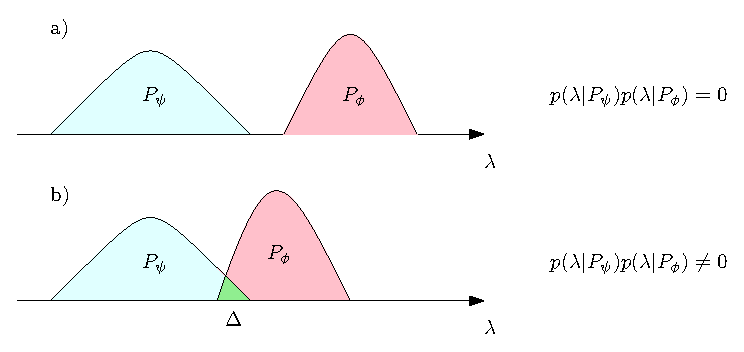
\includegraphics[scale=.7]{ontic}
\caption{\footnotesize{Harrigan and Spekkens' distinction between $\psi$-ontic (a) and $\psi$-epistemic (b) ontological models.}}\label{overlap}
\end{figure}

\section{Entropy and the ontological model}

To reproduce quantum theory, an ontological model has to reproduce not simply the probability of transitions during measurements but also all the results of quantum statistical mechanics and quantum information theory. Therefore, among other things, it has to obtain the correct values for entropy of mixed states. \textcolor{blue}{The natural way is by using standard information theoretic tools over the space of epistemic states which, as we will see, rules out $\psi$-ontic models. The degree of overlap between distributions, in fact, is not a choice, but is fixed by the value of entropy.} %@Gabriele: expand these points, i.e. explain more clearly the inference that you have in mind.

Let us first review a crucial property of the information entropy, both in the classical setting (i.e.\ the Shannon/Gibbs entropy) and in the quantum setting (i.e.\ the von Neumann entropy).\footnote{We show the explicit calculations in the appendix.} %@ Gabriele: why is it important to introduce both classical and quantum property of information entropy? Questi sono tutti commenti anti-referee. Esplicita meglio a cosa servono queste cose. 

\textbf{Classical information entropy of mixed non-overlapping distributions}. Let $\rho_1$ and $\rho_2$ be two classical distributions over a space $\Lambda$ with measure $\lambda$. The entropy for each distribution is given by the usual formula\footnote{The logarithm is assumed to be in base 2.}, for example
\begin{equation}\label{shannon_entropy}
	H(\rho_1) = - \int_\Lambda \rho_1(\lambda) \log \rho_1(\lambda) d\lambda.
\end{equation}
Suppose the two distributions are disjoint, and let $\rho = \frac{1}{2} \rho_1 + \frac{1}{2} \rho_2$ be a uniform mixture of the two distributions. The entropy of $\rho$ is given by
\begin{equation}\label{entropy_nonoverlap}
	H(\rho) = 1 + \frac{1}{2} H(\rho_1) + \frac{1}{2} H(\rho_2).
\end{equation}
Note how the non-overlapping assumption fixes the entropy of the mixed state.

\textbf{Quantum information entropy of quantum mixed states}. Now suppose $\psi$ and $\phi$ are two pure quantum states and let $p = | \langle \psi | \phi \rangle |^2$ be the probability of transition from one to the other. Consider the mixed state $\rho = \frac{1}{2} | \psi \rangle \langle \psi | + \frac{1}{2} | \phi \rangle \langle \phi |$. Its entropy is given by
\begin{equation}\label{entropy_mixed}
	H(\rho) = H\left(\frac{1+\sqrt{p}}{2}, \frac{1-\sqrt{p}}{2}\right).
\end{equation}

\textbf{Theorem: Since non-overlapping distributions can only represent orthogonal states, $\psi$-ontic models cannot be consistent with quantum theory.}

\emph{Proof}: Suppose we have a $\psi$-ontic model defined according to \cite{Harrigan:2010}. The epistemic states $p(\lambda|P_\psi)$ and $p(\lambda|P_\phi)$ consist of non-overlapping distributions over a space $\Lambda$,  \textcolor{blue}{therefore eq. \ref{entropy_nonoverlap} applies}. %@Gabriele: mi rendo conto che � stupido ma � un commento anti-referee. Tu dici che l'eq. 7 che riguarda distribuzioni classiche si applica al nostro caso che riguarda stati quantistici. Esplicita a prova di referee perch� si applica l'eq. 7 e non 8
Given that $\psi$ and $\phi$ are pure states, and the entropy for pure states is zero, we must have
\begin{equation}\label{entropy_pure}
	H(p(\lambda|P_\psi)) = H(p(\lambda|P_\phi)) = 0,
\end{equation}
and therefore
\begin{equation}\label{required_entropy}
	\begin{aligned}
		H\left(p(\lambda|\frac{1}{2}P_\psi + \frac{1}{2}P_\phi)\right) &= \\
		H\left(\frac{1}{2}p(\lambda|P_\psi) + \frac{1}{2}p(\lambda|P_\phi)\right) 
		&= 1.
	\end{aligned}
\end{equation}
If we compare the above with eq.~\ref{entropy_mixed}, it follows that $p$ must be zero. That is, we must have that
\begin{equation}\label{orthogonal}
	\langle \psi | \phi \rangle = 0
\end{equation}
no matter what $\psi$ and $\phi$ are.

Hence, the non-overlapping assumption built into the $\psi$-ontic model necessarily implies that all pure states are orthogonal. Since this is not true in quantum mechanics, any $\psi$-ontic model will fail to reproduce the results of quantum information, quantum statistical mechanics and, therefore, quantum theory in general. $\square$

We should also note that one has problems for $\psi$-epistemic models. While PBR leaves the possibility of $\psi$-epistemic models that use correlations, the correlations is also fixed by the entropy. %Commenti anti-reviewer: what do you mean here exactly when you speak about correlations? Do you know the existence of one of these models?
It is a well-known result in both classical and quantum information theory that \textcolor{red}{the entropy of a joint distribution of the marginal if and only if the subsystems are independent} (\cite{Ash:2010}, \cite{Nielsen:2010}). %@Gabriele: a verb seems to be missing in the red sentence.
Therefore an epistemic state that represents independent quantum states must also be the joint distribution of statistically independent epistemic states of the individual systems. This, combined with PBR, tells us that no models can reproduce quantum statistical mechanics and quantum information theory.

Thus, one concludes the following:
\begin{quote}
	\textbf{no ontological model can reproduce quantum statistical mechanics and quantum information with standard information theoretic tools}.
\end{quote}
That is, even if one had an ontological model that mapped the result of single outcome correctly, it would still give the wrong answer when trying to calculate ensembles and their entropy.

In principle, we do not exclude that someone may find a different construction to reproduce the correct entropies. There are, however, at least two objective difficulties that cannot be circumvented. First of all, information entropy is strictly concave, meaning that $H(p \rho_1 + (1-p) \rho_2) \geq p H(\rho_1) + (1-p) H(\rho_2)$ with the equality valid only if $\rho_1$ and $\rho_2$ are the same exact state. \textcolor{blue}{Therefore entropy fixed equality}. %spiega meglio
Because the mapping between epistemic states and density matrices is not injective,\footnote{Quantum mixture do not have a single decomposition in pure states. For example, the maximally mixed state of a qubit can be achieved with either an equal mixture of spin up and down or an equal mixture of spin left and right.} epistemic states must form equivalence classes and the strict concavity must be lost. That is, one can make mixtures of different ensemble without increasing entropy.

Secondly, as equation \ref{entropy_mixed} shows, the compute of the entropy requires the inner product. Therefore, whatever other structure one puts on top of epistemic states, essentially redefines the inner product. In other words, the idea that the inner product just represents transition probabilities, which, in our view, is the key idea the ontological model uses to explain ``what really happens'' does not work.

It is worth stressing, however, that it is not our task to solve these problems since we are neither the proponents of this model, nor supporters of it. Our only aim is to underline that the HS framework, as it currently stand, is highly problematic to draw any conclusion about the interpretation of quantum theory and the nature of $\psi$.

\section{Conclusion}

In this paper we proved that $\psi$-ontic models are not compatible with quantum information theory, and therefore with quantum mechanics itself.

One may think that the issue could be circumvented by substituting the Shannon entropy formula. %with what? 
That is, the problem would not be with the non-overlapping assumption made by HS but rather with how the entropy is calculated. However, the link between probability theory, information theory and measure theory is so tight that it makes this objection untenable. If we take a set of states $U$ with a measure $\mu(U)$ that quantifies the states in the set, the probability of each state for a uniform distribution is given by $\rho = 1 / \mu(U)$ and the entropy by $\log \mu(U)$. The measure used to count states, the probabilities assigned to states and the entropy assigned to distributions are not independent mathematical structures: failure of one entails the failure of all. We will look deeper into this issue in a later work.

Finally, combining our result with the PBR theorem it follows that both $\psi$-ontic and $\psi$-epistemic models cannot reproduce QM, contradicting the results and the predictions of quantum theory. This fact shows in turn that HS categorization of ontological models is fundamentally empty. Thus, such a framework should be employed neither to classify quantum interpretations, nor to draw conclusions on the nature of the quantum state.

Referring to this, being the HS definitions inadequate to reproduce QM, it follows that any result derived from them rests on a technically ill-defined basis, as for instance the PBR theorem itself. If this is true, then, it is not demonstrated (i) that quantum states must necessarily be HS-$\psi$-ontic, and (ii) that HS-$\psi$-epistemic interpretations are contradicted by quantum theory. Concluding, we believe that the PBR theorem does not make claims on the reality of the quantum state, but it rather shows that HS definition of $\psi$-epistemic model contradicts QM. If interpreted in this manner, the PBR result is the first part of a more general argument showing the inadequacy of the HS framework to categorize quantum theories. Argument that we have completed with the proposed no-go theorem against $\psi$-ontic models.

\section{Acknowledgements}

Andrea Oldofredi is grateful to the Funda\c{c}$\tilde{\mathrm{a}}$o para a Ci\^encia e a Tecnologia (FCT) for financial support (Grant no. 2020.02858.CEECIND).  This work is in connection to Assumptions of Physics, a larger project that aims to identify a handful of physical principles from which the basic laws can be rigorously derived  (\url{https://assumptionsofphysics.org}).

%\bibliographystyle{ieeetr}
\bibliography{bibliography}
\clearpage

\section*{Appendix: calculation}
\label{A}
\textbf{Entropy of mixed non-overlapping distributions}. We want to show that, given two non-overlapping probability distributions $\rho_1$ and $\rho_2$, the entropy of $\rho = \frac{1}{2} \rho_1 + \frac{1}{2} \rho_2$ is given by
\begin{equation}
	H(\rho) = 1 + \frac{1}{2} H(\rho_1) + \frac{1}{2} H(\rho_2). \tag{\ref{entropy_nonoverlap}}
\end{equation}

Let $U_1, U_2 \subset \Lambda$ be the respective supports of the distributions, which are non-overlapping i.e.\ $U_1 \cap U_2 = \emptyset$. We then have
\begin{align*}
	H(\rho) &= - \int_\Lambda \rho \log \rho d\lambda \\
	&= -\int_{U_1} \rho \log \rho d\lambda -\int_{U_2} \rho \log \rho d\lambda \\
	&= -\int_{U_1} \frac{1}{2} \rho_1 \log \frac{1}{2} \rho_1 d\lambda -\int_{U_2} \frac{1}{2} \rho_2 \log \frac{1}{2} \rho_2 d\lambda \\
	&= - \frac{1}{2} \int_{U_1} \rho_1 \log \frac{1}{2} d\lambda - \frac{1}{2} \int_{U_1} \rho_1 \log \rho_1 d\lambda \\
	&- \frac{1}{2} \int_{U_2} \rho_2 \log \frac{1}{2} d\lambda - \frac{1}{2} \int_{U_2} \rho_2 \log \rho_2 d\lambda \\
	&= - \frac{1}{2} \log \frac{1}{2} - \frac{1}{2} \log \frac{1}{2} + \frac{1}{2} H(\rho_1) + \frac{1}{2} H(\rho_2) \\
	&= 1 + \frac{1}{2} H(\rho_1) + \frac{1}{2} H(\rho_2). \\
\end{align*}


\textbf{Entropy of quantum mixed states}. We want to show that, given two states $\psi$ and $\phi$, the entropy of the mixed state $\rho = \frac{1}{2}|\psi\rangle\langle\psi| + \frac{1}{2}|\phi\rangle\langle\phi|$ is
\begin{equation}\label{entropy}
	H(\rho) = H\left(\frac{1+|\langle\psi|\phi\rangle|}{2}, \frac{1-|\langle\psi|\phi\rangle|}{2}\right).
\end{equation}

\begin{center}
	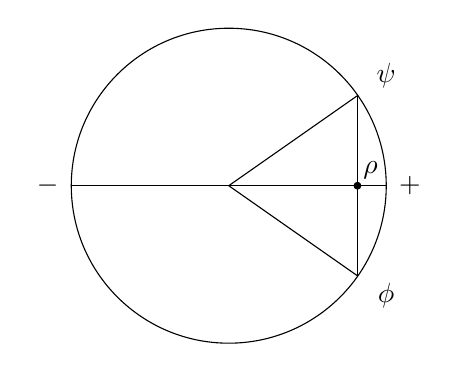
\begin{tikzpicture}[scale = 1]
		\draw (0,0) circle (2);
		\node at (-2.3,0) {$-$};
		\node at (2.3,0) {$+$};
		\node at (2,1.4) {$\psi$};
		\node at (2,-1.4) {$\phi$};
		\draw (-2,0) -- (2,0);
		\begin{scope}
			\clip(0,0) circle (2);
			\draw (0,0) -- (2,1.4);
			\draw (0,0) -- (2,-1.4);
			\draw (1.634,1.4) -- (1.634,-1.4);
		\end{scope}
		\fill (1.634,0) circle (0.05);
		\node at (1.8,.2) {$\rho$};
	\end{tikzpicture}
\end{center}

Note that $\psi$ and $\phi$ will identify a two-dimensional subspace which can be thought, without loss of generality, as a qubit and therefore can be represented by a Bloch sphere. The picture represents the intersection of the Bloch sphere with the plane identified by $\psi$ and $\phi$. As $\rho$ is an equal mixture of the two states, it will be represented by the midpoint between the two. Taking the line that goes through $\rho$ and the center of the sphere, we can see that $\rho$ can also be seen as the mixture of the states $+$ and $-$ which, since they represent equal and opposite directions, form a basis. To diagonalize $\rho$, then, means to express it in terms of $+$ and $-$.

If $\theta_{\psi\phi}$ is the angle between $\psi$ and $\phi$, we have
\begin{equation}
	|\langle \psi | \phi \rangle |^2 = \cos^2 \frac{\theta_{\psi\phi}}{2}.
\end{equation}
The angle is divided by two because the angle on the Bloch sphere (i.e. in physical space) is double the angle in the Hilbert space. For example, for $z^+$ and $z^-$ the angle on the Bloch sphere would be $\pi$ and the inner product is zero (i.e. opposite directions in physical space correspond to orthogonal states).

Now we express $\psi$ and $\phi$ in terms of $+$ and $-$, remembering that they form a basis. Given that $\rho$ is at the midpoint, the figure is vertically symmetric. The angle between $\psi$ and $+$, then, is half of $\theta_{\psi\phi}$. The inner product between $\psi$ and $+$ is
\begin{equation}
	\begin{aligned}
		|\langle \psi | + \rangle |^2 &= \cos^2 \frac{\theta_{\psi +}}{2} \\
		&= \cos^2 \frac{\theta_{\psi\phi}}{4}.
	\end{aligned}
\end{equation}
Keeping in mind that we are composing vectors in the Hilbert space (and not in the geometry of the physical space) we have
\begin{align*}
	\left|\psi\right>&=\cos\frac{\theta_{\psi\phi}}{4}\left|+\right>+\sin\frac{\theta_{\psi\phi}}{4}\left|-\right> \\
	\left|\phi\right>&=\cos\frac{\theta_{\psi\phi}}{4}\left|+\right>-\sin\frac{\theta_{\psi\phi}}{4}\left|-\right>.
\end{align*}

The density matrices corresponding to the pure states are
\begin{align*}
	\left|\psi\right>\left<\psi\right|&=\cos^2\frac{\theta_{\psi\phi}}{4}\left|+\right>\left<+\right|\\
	&+\cos\frac{\theta_{\psi\phi}}{4}\sin\frac{\theta_{\psi\phi}}{4}\left(\left|+\right>\left<-\right|+\left|-\right>\left<+\right|\right) \\
	&+\sin^2\frac{\theta_{\psi\phi}}{4}\left|-\right>\left<-\right| \\
	\left|\phi\right>\left<\phi\right|&=\cos^2\frac{\theta_{\psi\phi}}{4}\left|+\right>\left<+\right|\\
	&-\cos\frac{\theta_{\psi\phi}}{4}\sin\frac{\theta_{\psi\phi}}{4}\left(\left|+\right>\left<-\right|+\left|-\right>\left<+\right|\right) \\
	&+\sin^2\frac{\theta_{\psi\phi}}{4}\left|-\right>\left<-\right|.
\end{align*}

We can now calculate the mixture
\begin{align*}
	\frac{1}{2}(|\psi\rangle\langle\psi| &+ |\phi\rangle\langle\phi|) \\
	&=\cos^2\frac{\theta_{\psi\phi}}{4}\left|+\right>\left<+\right| +\sin^2\frac{\theta_{\psi\phi}}{4}\left|-\right>\left<-\right| \\
	&=\frac{1+\cos\frac{\theta_{\psi\phi}}{2}}{2}\left|+\right>\left<+\right| +\frac{1-\cos\frac{\theta_{\psi\phi}}{2}}{2}\left|-\right>\left<-\right| \\
	&=\frac{1+|\langle\psi|\phi\rangle|}{2}\left|+\right>\left<+\right| +\frac{1-|\langle\psi|\phi\rangle|}{2}\left|-\right>\left<-\right|. \\
\end{align*}

As $\rho$ is in a diagonal form, the entropy is given by \ref{entropy}.


\end{document}